\subsection{\texorpdfstring{连续映射空间中的 \(\mathfrak{S}\)-收敛}{连续映射空间中的 S-收敛}}

设 X、Y 为两个拓扑空间，用 C(X; Y) 表示由 X 到 Y 中的全体连续映射所成之集。若 S 是 X 的子集所成之集，且 Y 是一致空间，则用 \(\mathcal{C}_{\mathfrak{S}}(\mathbf{X};\mathbf{Y})\) 表示赋有 S-收敛一致结构的集合 C(X; Y)。特别地，\(\mathcal{C}_{s}(\mathbf{X};\mathbf{Y})\) 、\(\mathcal{C}_{c}(\mathbf{X};\mathbf{Y})\) 与 \(\mathcal{C}_{u}(\mathbf{X};\mathbf{Y})\) 分别表示赋有逐点收敛、紧收敛与一致收敛一致结构的集合 C(X; Y)。

命题 6. 设 X 是拓扑空间，Y 是一致空间，S 是 X 的子集所成之集。对每个 A ∈ S 以及 Y 的每个闭围域 V，W(A, V) 与 W(A̅, V) 在 C (X; Y) × C (X; Y) 上的迹相同。

因为若 \(u, v\) 是 \(\mathbf{X}\) 到 \(\mathbf{Y}\) 中的连续映射，则映射 \(x \to (u(x), v(x))\) 把 \(\mathbf{X}\) 映入 \(\mathbf{Y} \times \mathbf{Y}\) 并且连续，于是由 \((u(x), v(x)) \in \mathbf{V}\) 对一切 \(x \in \mathbf{A}\) 成立这一假设便可推出，\((u(x), v(x)) \in \overline{\mathbf{V}} = \mathbf{V}\) 对一切 \(x \in \overline{\mathbf{A}}\) 成立（第 I 章，§ 2，第 1 号，定理 1）。

若用 \(\overline{\mathfrak{S}}\) 表示在 \(\mathbf{X}\) 中所取的 \(\mathfrak{S}\) 的诸集的闭包所成之集，则命题 6 表明，在 \(\mathcal{C}(\mathbf{X};\mathbf{Y})\) 上，\(\mathfrak{S}\) -收敛与 \(\overline{\mathfrak{S}}\) -收敛的结构相同。

推论. 设 B 是 X 的稠密子集。在 C(X; Y) 上，一致收敛的结构与 B 上的一致收敛的结构相同。

命题 7. 设 X 是拓扑空间，S 是 X 的子集所成之集，Y 是一致空间。若 Y 是豪斯多夫空间，且 S 中诸集的并 B 在 X 中稠密，则 \(\mathcal{C}_{\mathfrak{S}}(X;Y)\) 是豪斯多夫空间。

因为若 \((u, v)\) 属于所有的集 \(W(A, V)\) ，其中 \(A \in \mathfrak{S}\) 而 \(V\) 取遍 \(Y\) 的围域，则由 \(Y\) 是豪斯多夫空间这一假设知，\(u(x) = v(x)\) 对一切 \(x \in B\) 成立；若 \(u\) 与 \(v\) 连续，则由恒等延拓原理得 \(u = v\)（第 I 章，§ 8，第 1 号，命题 2 的推论 1）。

特别地，在 \(\mathcal{C}(\mathbf{X};\mathbf{Y})\) 上，\(\mathbf{X}\) 的一个稠密子集上的逐点收敛拓扑是豪斯多夫的。

命题 8. 设 X 是一个集合，F 是 X 上的滤子，Y 是一致空间。则由映射 \(u: \mathbf{X} \to \mathbf{Y}\) （其中 \(u(\mathfrak{F})\) 是 Y 上的柯西滤子基）所成之集 H 在 \(\mathcal{F}_u(\mathbf{X}; \mathbf{Y})\) 中是闭的。

设 \(u_0: \mathbf{X} \to \mathbf{Y}\) 属于 \(\mathbf{H}\) 在 \(\mathcal{F}_u(\mathbf{X}; \mathbf{Y})\) 中的闭包。设 \(\mathbf{V}\) 为 \(\mathbf{Y}\) 的任一对称围域，则存在映射 \(u \in \mathbf{H}\) ，使得 \((u_0(x), u(x)) \in \mathbf{V}\) 对一切 \(x \in \mathbf{X}\) 成立；另一方面，由假设存在集 \(\mathbf{M} \in \mathfrak{F}\) ，使得 \((u(x), u(x')) \in \mathbf{V}\) 每当 \(x\) 与 \(x'\) 都属于 \(\mathbf{M}\) 。由于 \((u_0(x), u(x)) \in \mathbf{V}\) 且 \((u_0(x'), u(x')) \in \mathbf{V}\) ，便得 \((u_0(x), u_0(x')) \in \overset{3}{\mathbf{V}}\) 每当 \(x\) 与 \(x'\) 都属于 \(\mathbf{M}\) ，从而 \(u_0(\mathfrak{F})\) 是 \(\mathbf{Y}\) 上的柯西滤子基。

推论 1. 设 X 是拓扑空间，Y 是一致空间。在一点 \(x_{0} \in X\) 处连续的、由 X 到 Y 中的映射所成之集在 \(\mathcal{F}_{u}(X; U)\) 中是闭的。

若 V 是 \(x_{0}\) 在 X 中的邻域滤子，则 \(u(x_{0})\) 是 \(u(\mathbf{V})\) 的接触点；因此 u 在 \(x_{0}\) 处连续当且仅当 \(u(\mathbf{V})\) 是 Y 上的柯西滤子基（第 II 章，§ 3，第 2 号，命题 5 的推论 2）。

推论 2. 设 X、L 为两个集合，分别带有滤子 F、G，并设 Y 是完备一致空间。对每个 \(\lambda \in L\) ，设 \(u_{\lambda}\) 是 X 到 Y 中的一个映射。假设：(i) 族 \((u_{\lambda})_{\lambda \in L}\) 在 X 中（关于滤子 G）一致收敛于映射 \(v: X \to Y\) ；(ii) 对每个 \(\lambda \in L\) ，\(u_{\lambda}\) 关于滤子 F 有极限 \(y_{\lambda}\) 。在这些条件下，\(v\) 关于 F 有极限，且 \(v\) 关于 F 的每个极限都是族 \((y_{\lambda})_{\lambda \in L}\) 关于 G 的极限。

因为 \(v\) 属于诸 \(u_{\lambda}\) 所成之集在 \(\mathcal{F}_u(\mathbf{X};\mathbf{Y})\) 中的闭包，故由命题 8 知 \(v(\mathfrak{F})\) 是 \(\mathbf{Y}\) 上的柯西滤子基；这表明 \(v\) 有极限 \(y\) （关于 \(\mathfrak{F}\) ），因为 \(\mathbf{Y}\) 是完备的。设

\(X' = X \cup \{\omega\}\) 为与滤子 \(\mathfrak{F}\) 相伴的拓扑空间（第 I 章，§ 6，第 5 号），并把 \(u_{\lambda}\) （相应地，\(v\) ）延拓为 \(\overline{u}_{\lambda}\) （相应地，\(\overline{v}\) ），即 \(X'\) 到 Y 中的映射，办法是令 \(\overline{u}_{\lambda}(\omega) = y_{\lambda}\) {[}相应地 \(\overline{v}(\omega) = y\) {]}。于是映射 \(\overline{u}_{\lambda}, \overline{v}\) 在 \(X'\) 上连续，且 \(\overline{u}_{\lambda}\) 在 X 中一致收敛于 \(\overline{v}\) （关于 \(\mathfrak{G}\) ）；由于 X 在 \(X'\) 中稠密，命题 6 的推论表明 \(\overline{u}_{\lambda}\) 在 \(X'\) 中一致收敛于 \(\overline{v}\) ，特别地有 \(y = \lim_{\mathfrak{G}} y_{\lambda}\) 。

定理 2. 设 X 是拓扑空间，Y 是一致空间。则由 X 到 Y 中的连续映射所成之集 C(X; Y) 是赋有一致收敛拓扑的空间 F(X; Y) 的闭子集。

对每个 \(x \in \mathbf{X}\) ，由 \(\mathbf{X}\) 到 \(\mathbf{Y}\) 中的、在 \(x\) 处连续的映射所成之集在 \(\mathcal{F}_u(\mathbf{X};\mathbf{Y})\) 中是闭的（命题 8 的推论 1）；因此这些集的交 \(\mathcal{C}(\mathbf{X};\mathbf{Y})\) 也是闭的。

这一结果可以表述为：连续函数的一致极限仍然连续。

推论 1. 若 Y 是完备一致空间，则 \(\mathcal{C}_{u}(\mathbf{X};\mathbf{Y})\) 是完备的。因为由定理 2，\(\mathcal{C}_{u}(\mathbf{X};\mathbf{Y})\) 是一致空间 \(\mathcal{F}_{u}(\mathbf{X};\mathbf{Y})\) 的闭一致子空间，而后者由第 5 号的定理 1 是完备的。

推论 2. 设 X 是拓扑空间，S 是 X 的子集所成之集，Y 是一致空间。用 \(\tilde{\mathcal{C}}_{\mathfrak{S}}(X;Y)\) 表示由其在 S 的每个集上的限制都连续的、X 到 Y 中的全体映射所成之集。则 \(\tilde{\mathcal{C}}_{\mathfrak{S}}(X;Y)\) 是一致空间 \(\mathcal{F}_{\mathfrak{S}}(X;Y)\) 的闭子空间，且当 Y 完备时它是完备的。

设 \(u\) 属于 \(\tilde{\mathcal{C}}_{\mathfrak{S}}(\mathbf{X};\mathbf{Y})\) 在 \(\mathcal{F}_{\mathfrak{S}}(\mathbf{X};\mathbf{Y})\) 中的闭包；则（第 2 号）对每个 \(\mathbf{A} \in \mathfrak{S}\) ，\(u|\mathbf{A}\) 属于 \(\mathcal{C}(\mathbf{A};\mathbf{Y})\) 在 \(\mathcal{F}_u(\mathbf{A};\mathbf{Y})\) 中的闭包，从而由定理 2 知它连续。

推论 3. 设 X 是可度量化或局部紧的拓扑空间，Y 是一致空间。则 \(\mathcal{C}(\mathbf{X};\mathbf{Y})\) 在一致空间 \(\mathcal{F}_c(\mathbf{X};\mathbf{Y})\) 中是闭的；若此外 Y 还是完备的，则一致空间 \(\mathcal{C}_c(\mathbf{X};\mathbf{Y})\) 是完备的。

由推论 2，只需证明：若取 \(\mathfrak{S}\) 为 X 的紧子集所成之集，则在所考虑的两种情形下都有 \(\tilde{\mathcal{C}}_{\mathfrak{S}}(X;Y) = \mathcal{C}(X;Y)\) 。若 X 局部紧，这是显然的。若 X 可度量化，且 \(u: X \to Y\) 是一个在每个紧子集上的限制都连续的映射，则对每个 \(x \in X\) 以及每个序列 \((z_n)\) （由 X 的点组成且收敛于 \(x\) ），有 \(u(x) = \lim_{n \to \infty} u(z_n)\) ，因此 \(u\) 在 \(x\) 处连续（第 IX 章，§ 2，第 6 号，命题 10）。

注意，只要 \(\mathbf{X}\) 的每一点都具有可数的基本邻域系，上面的论证就适用。

\pandocbounded{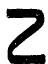
\includegraphics[keepaspectratio]{images/part002_71b18b59.jpg}}

注。1) 一般说来，集 \(\mathcal{C}(\mathbf{X};\mathbf{Y})\) 关于逐点收敛拓扑在 \(\mathcal{F}(\mathbf{X};\mathbf{Y})\) 中不是闭的：换句话说，连续函数的逐点极限未必连续{[}习题 5 a){]}。

\begin{enumerate}
\def\labelenumi{\arabic{enumi})}
\setcounter{enumi}{1}
\tightlist
\item
  \(\mathcal{C}(\mathbf{X};\mathbf{Y})\) 上的一个滤子可以逐点收敛于一个连续函数而不一致收敛于这个函数。
\end{enumerate}

例如，在区间 I = {[}0, 1{]} 上，设 \(u_n\) 是这样的实值函数：当 \(x = 0\) 且 \(2/n \leqslant x \leqslant 1\) 时等于 0，当 \(x = 1/n\) 时等于 1，并且在区间 {[}0, 1/n{]} 与 {[}1/n, 2/n{]} 的每一个中都是线性的。序列 \((u_n)\) 逐点收敛于 0，但在 I 中不一致收敛于 0（参见习题 6）。

\begin{enumerate}
\def\labelenumi{\arabic{enumi})}
\setcounter{enumi}{2}
\item
  若 X 是一致空间，则与命题 8 类似的证明表明，由 X 到 Y 中的一致连续映射所成之集在 \(\mathcal{F}_u(X;Y)\) 中是闭的。
\item
  设一致空间 Y 带有一个交换且结合的合成律，用加法记写，使得映射 \((y, y') \to y + y'\) 在 \(Y \times Y\) 上连续。于是，若 \((u_n)\) 是 X 到 Y 中的连续映射序列，且以 \(u_n\) 为通项的级数在 X 中一致收敛，则该级数的和在 X 上连续。
\end{enumerate}

关于连续映射的一致可和族（第 1 号，注 5）的相应结果，留给读者自行叙述。

命题 9. 设 X 是拓扑空间，Y 是一致空间。则映射 \((f, x) \to f(x)\) （由 \(\mathcal{C}_u(X; Y) \times X\) 到 Y 中）是连续的。

设 \(f_0: \mathbf{X} \to \mathbf{Y}\) 是连续映射，\(x_0\) 是 \(\mathbf{X}\) 的一点，\(\mathbf{V}\) 是 \(\mathbf{Y}\) 的一个围域。集 \(\mathbf{T}\) 由诸连续映射 \(f: \mathbf{X} \to \mathbf{Y}\) 组成，它们满足 \((f(x), f(x_0)) \in \mathbf{V}\) 对一切 \(x \in \mathbf{X}\) 成立；这个集是 \(f_0\) 在 \(\mathcal{C}_u(\mathbf{X}; \mathbf{Y})\) 中的一个邻域。另一方面，由于 \(f_0\) 连续，存在一个邻域 \(\mathbf{U}\) （\(x_0\) 在 \(\mathbf{X}\) 中的邻域），使得 \((f_0(x), f_0(x_0)) \in \mathbf{V}\) 对一切 \(x \in \mathbf{U}\) 成立。因此我们有 \((f(x), f(x_0)) \in \overset{\circ}{\mathbf{V}}\) 每当 \((f, x) \in \mathbf{T} \times \mathbf{U}\) ，从而结论得证。

